\documentclass[aspectratio=169]{beamer}
\usetheme{metropolis}
% Temple University Color Scheme
\definecolor{TempleCherry}{RGB}{164,30,53}
\definecolor{TempleWhite}{RGB}{255,255,255}
\definecolor{TempleGray}{RGB}{100,100,100}

\setbeamercolor{structure}{fg=TempleCherry}
\setbeamercolor{palette primary}{bg=TempleCherry,fg=TempleWhite}
\setbeamercolor{palette secondary}{bg=TempleCherry!80,fg=TempleWhite}
\setbeamercolor{palette tertiary}{bg=TempleCherry!60,fg=black}
\setbeamercolor{titlelike}{bg=TempleWhite,fg=TempleCherry}
\setbeamercolor{frametitle}{bg=TempleCherry,fg=TempleWhite}
\setbeamercolor{block title}{bg=TempleCherry,fg=TempleWhite}
\setbeamercolor{block body}{bg=TempleCherry!10,fg=black}

% Packages
\usepackage{amsmath}
\usepackage{amssymb}
\usepackage{bm}
\usepackage{graphicx}
\usepackage{booktabs}
\usepackage{subcaption}
\usepackage{tikz}
\usepackage{algorithm}
\usepackage{algorithmic}
\usetikzlibrary{positioning,shapes.geometric,arrows.meta}

% Graphics path
\graphicspath{{figures/}}

% Bibliography
\usepackage[style=apa,natbib=true]{biblatex}
\addbibresource{references.bib}

% Presentation metadata
\title[MEMS-GeoNav: UKF]{\textcolor{black}{Navigation in GNSS-Denied Environments Using MEMS-Grade Sensors and Geophysical Anomalies: A UKF Approach}}
\subtitle{\textcolor{black}{ION International Technical Meeting 2026}}
\author{James Brodovsky \and Philip Dames}
\institute{Temple University}
\date{28 January 2026}


% Logo placeholder - uncomment when available
% \titlegraphic{\includegraphics[width=2cm]{example-image-a}}

\begin{document}

% ============================================================
% TITLE SLIDE
% ============================================================
\begin{frame}
\titlepage
\end{frame}

% ============================================================
% OUTLINE
% ============================================================
\begin{frame}{Outline}
\tableofcontents
\end{frame}

% ============================================================
\section{Introduction}
% ============================================================

% ============================================================
% MOTIVATION: GNSS VULNERABILITIES
% ============================================================
\begin{frame}{The GNSS Dependency Problem}
    \textbf{Modern navigation is critically dependent on GNSS which creates a single point of failure that can be disrupted in many ways.}
    \vspace{1cm}
    \pause
\begin{columns}[t]
\begin{column}{0.5\textwidth}
\textbf{Natural Degradation:}
\begin{itemize}
    \item Urban canyons \& multipath
    \item Indoor/underground environments
    \item Underwater operations
    \item Ionospheric disturbances and solar weather
\end{itemize}
\pause
\end{column}
\begin{column}{0.5\textwidth}
\textbf{Intentional Disruption:}
\begin{itemize}
    \item Electronic warfare (jamming)
    \item GNSS spoofing attacks
    \item Critical for aviation, maritime, military
\end{itemize}
\end{column}
\end{columns}

\vspace{0.25cm}
\centering
\begin{alertblock}{\textcolor{white}{Solution Needed}}
Alternative PNT (Alt-PNT) solutions that do not rely on external RF signals
\end{alertblock}
\end{frame}

% ============================================================
% MOTIVATION: COST GAP & GEOPHYSICAL NAVIGATION
% ============================================================
\begin{frame}{Geophysical Navigation: The Cost-Performance Gap}
\begin{columns}[t]
\begin{column}{0.5\textwidth}
\textbf{Core Concept:}
\begin{itemize}
    \item Exploit naturally occurring variations in Earth's physical fields
    \item Gravity and magnetic anomalies are spatially correlated
    \item Maps available for reference
    \item Passive, non-RF alternative
\end{itemize}
\pause
\textbf{Historical Approaches:}
\begin{itemize}
    \item Navigation/Tactical-grade IMUs with dedicated gravimeters and magnetometers
    \item Cost: \$10K - \$100K+
    \item Military \& aerospace applications
\end{itemize}
\end{column}
\begin{column}{0.5\textwidth} \pause
\textbf{Potential Impact:} Extends alt-PNT geophysical navigation to new domains
\begin{itemize}
    \item Commercial drones
    \item Small autonomous vehicles
    \item Low SWaP constraints
\end{itemize}
\end{column}
\end{columns}
\end{frame}
% ============================================================
% RESEARCH OBJECTIVE
% ============================================================
\begin{frame}{Research Objective}
    \centering
    \textbf{Can we extend geophysical navigation to low-Size Weight and Power (SWaP) mass-market platforms?}
\end{frame}

% ============================================================
\section{Methodology}
% ============================================================

% ============================================================
% DATASET
% ============================================================
\begin{frame}{MEMS-Nav Dataset}
\begin{columns}
\begin{column}{0.55\textwidth}
\textbf{Data Collection:}
\begin{itemize}
    \item Smartphone-grade MEMS sensors
    \item Highway driving scenarios
    \item 30 minutes to several hours each
    \item Tens to hundreds of kilometers
\end{itemize}
\pause
\textbf{Sensor Suite:}
\begin{itemize}
    \item 3-axis accelerometer (m/s$^2$)
    \item 3-axis gyroscope (rad/s)
    \item 3-axis magnetometer ($\mu$T)
    \item GNSS receiver (lat, lon, alt, velocity)
    \item Barometric altimeter
\end{itemize}
\end{column}
\begin{column}{0.45\textwidth}
\centering
% Placeholder for trajectory map
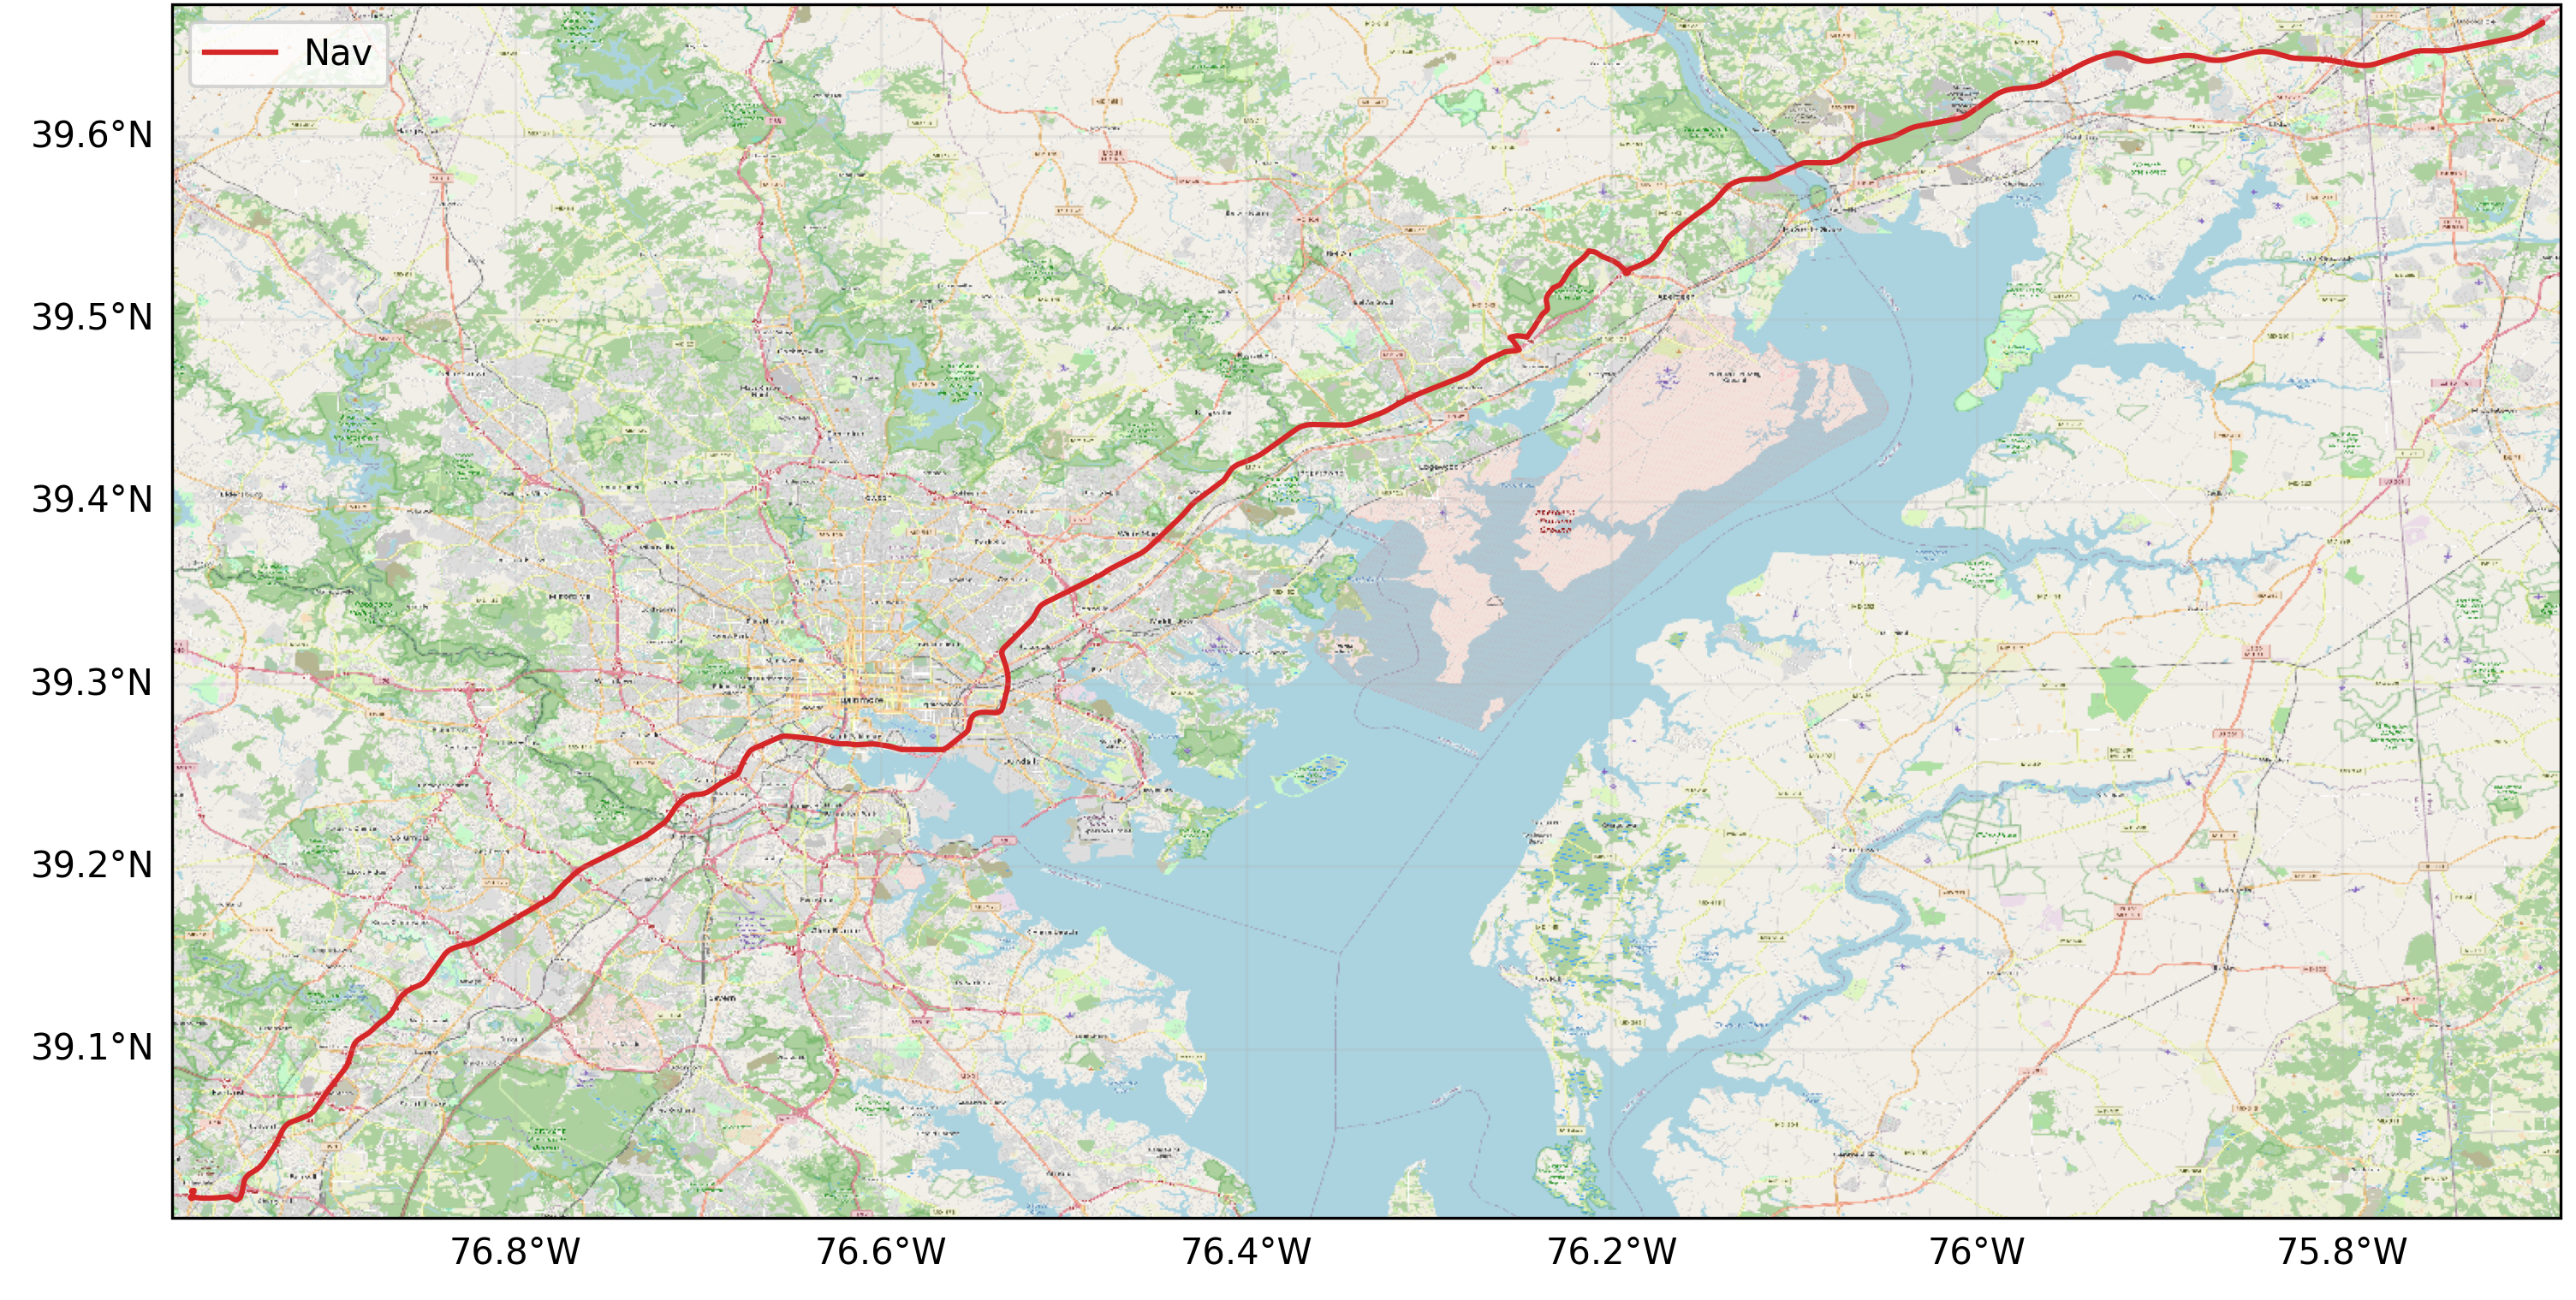
\includegraphics[width=\textwidth]{example_street_map.png}
\small
\textit{An example trajectory from the MEMS-Nav dataset}
\end{column}
\end{columns}
\end{frame}

% ============================================================
% SYSTEM ARCHITECTURE
% ============================================================
\begin{frame}{System Architecture}
\centering
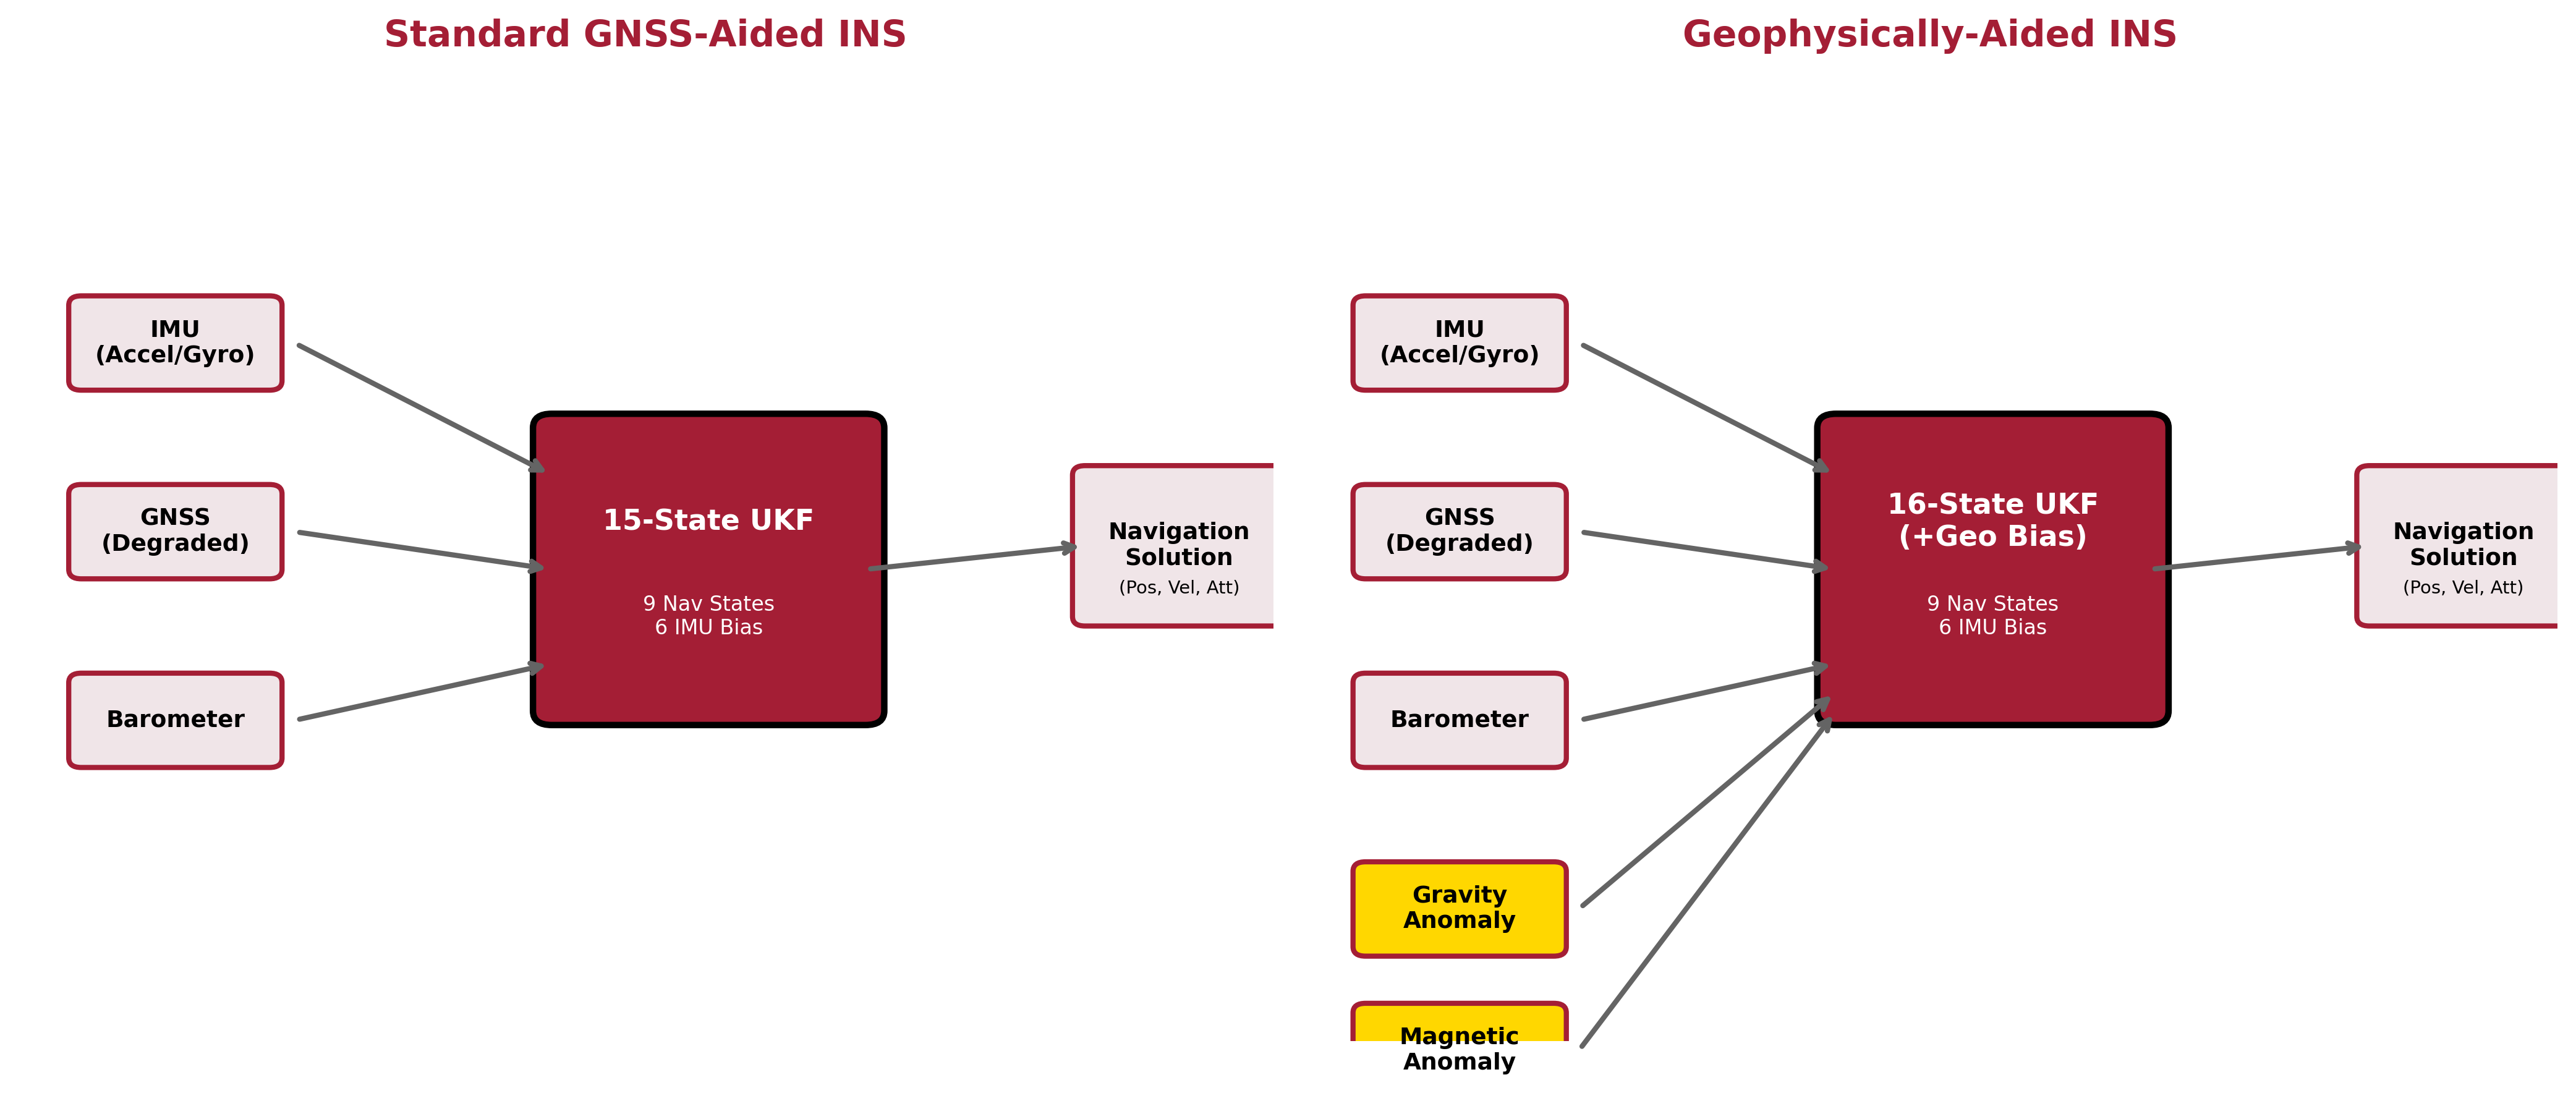
\includegraphics[width=0.85\textwidth]{system_architecture.png}

\vspace{0.5cm}
\textbf{15-State UKF INS} + Geophysical Augmentation
\end{frame}

% ============================================================
% STATE VECTOR
% ============================================================
\begin{frame}{Standard 15-State UKF INS}
\textbf{State Vector (15 states):}
\begin{equation*}
\mathbf{x} = \left[\begin{array}{ccccccccccccccc}
  L & \lambda & h & v_n & v_e & v_d & \phi & \theta & \psi & b_{a_x} & b_{a_y} & b_{a_z} & b_{g_x} & b_{g_y} & b_{g_z}
\end{array}\right]^\intercal
\end{equation*}

\vspace{0.5em}

\begin{columns}[t]
\begin{column}{0.3\textwidth}
\textbf{Position (LLF):}
\begin{itemize}
    \item $L$ - Latitude
    \item $\lambda$ - Longitude
    \item $h$ - Altitude (MSL)
\end{itemize}
\end{column}

\begin{column}{0.3\textwidth}
\textbf{Velocity (NED):}
\begin{itemize}
    \item $v_n$ - North
    \item $v_e$ - East
    \item $v_d$ - Down
\end{itemize}
\end{column}

\begin{column}{0.4\textwidth}
\textbf{Attitude + Biases:}
\begin{itemize}
    \item $\phi, \theta, \psi$ - Roll, Pitch, Yaw
    \item $\mathbf{b}_a$ - Accel biases
    \item $\mathbf{b}_g$ - Gyro biases
\end{itemize}
\end{column}
\end{columns}

\vspace{1em}

\textbf{Propagation:} Strapdown mechanization equations (Groves Ch. 5)

\textbf{Updates:} GNSS position/velocity + barometric altitude
\end{frame}

% ============================================================
% GNSS DEGRADATION SCENARIO
% ============================================================
\begin{frame}{GNSS Degradation Scenario}
\begin{columns}[t]
\begin{column}{0.5\textwidth}
\textbf{AR(1) Correlated Errors:}
\begin{itemize}
    \item Position: $\rho_{\text{pos}} = 0.99$, $\sigma_{\text{pos}} = 5$ m
    \item Velocity: $\rho_{\text{vel}} = 0.95$, $\sigma_{\text{vel}} = 5$ m/s
    \item Slowly drifting biases (not white noise)
    \item Models multipath/atmospheric delays
\end{itemize}
\pause
\end{column}
\begin{column}{0.5\textwidth}
    \textbf{Covariance Inflation:}
    \begin{itemize}
        \item Scale factor: $r_{\text{scale}} = 15$
        \item $15\times$ advertised accuracy
        \item Simulates poor DOP reporting
        \item Filter trusts GNSS less
    \end{itemize}
    \pause
\end{column}
\end{columns}
\vspace{.25cm}
\begin{alertblock}{\textbf{\textcolor{white}{Challenge}}}
Combination of correlated errors + inflated covariance stresses filter's ability to maintain accurate state estimates
\end{alertblock}

\vspace{0.5em}
\textbf{Applied identically} to both baseline and geophysically-aided systems

\end{frame}

% ============================================================
% GEOPHYSICAL AIDING
% ============================================================
\begin{frame}{Geophysical Measurement Model}
% \begin{columns}[t]
% \begin{column}{0.5\textwidth}
\textbf{Anomaly Maps:}
\begin{itemize}
    \item \textbf{Gravity:} IGPP Earth Free-air Anomaly, 1 arc-minute resolution ($\sim$1.8 km)
    \item \textbf{Magnetic:} WDMAM, 3 arc-minute resolution ($\sim$5.6 km)
    \item Accessed via GMT software
    \item Bilinear interpolation
\end{itemize}
\pause
\textbf{Processing:}
\begin{enumerate}
    \item Measure gravity/magnetic field
    \item Subtract theoretical model
    \item Compare residual to anomaly map
    \item Add bias state to UKF (16 states)
\end{enumerate}
\end{frame}

\begin{frame}{Geophysical Measurement Model}
\begin{columns}[t]
\begin{column}{0.5\textwidth}
\textbf{Generalized Measurement Model:}
\begin{equation*}
h(\mathbf{x}) = \text{map}(L, \lambda) + \mathcal{N}(0, \sigma_{\text{geo}})
\end{equation*}
\begin{table}[h]
    \centering
    \small
    \caption{Measurement residual distributions}
    \begin{tabular}{lcc}
        \toprule
        Anomaly Type & Mean & Std. Dev \\
        \midrule
        Gravity & 5.97 mGal & 48.93 mGal\\
        Magnetic & 40,364 nT & 41,303 nT\\
        \bottomrule
    \end{tabular}
\end{table}
\end{column}
\begin{column}{0.5\textwidth}
\textbf{Measurement Noise Parameters:}

\includegraphics[width=\textwidth]{anomaly_differences.png}
\end{column}
\end{columns}

\end{frame}

% ============================================================
\section{Results}
% ============================================================

% ============================================================
% PERFORMANCE EVALUATION
% ============================================================
\begin{frame}{Performance Evaluation}
\textbf{Three Configurations Tested:}
\begin{enumerate}
    \item Standard GNSS-aided INS (degraded GNSS baseline)
    \item GNSS + Gravity anomaly aiding
    \item GNSS + Magnetic anomaly aiding
\end{enumerate} \pause
\textbf{Error Metrics:}
\begin{itemize}
    \item Haversine distance (great-circle distance on sphere)
    \item Altitude difference
    \item Compare estimated position to reference GNSS
    \item $\Delta$ Error = Geophysical Error - Baseline Error; negative values indicate improvement
\end{itemize} \pause
\textbf{Statistics:} RMSE, Mean, Median position error; individual and aggregated across 13 trajectories
\end{frame}

% ============================================================
% SUMMARY STATISTICS
% ============================================================
\begin{frame}{Summary Statistics Across All Trajectories}
\begin{table}
    \scriptsize
    \centering
    \begin{tabular}{ || l  ||ccc|| ccc|| }
    \toprule
   Trajectory & \multicolumn{3}{c||}{Gravity Aiding}& \multicolumn{3}{c||}{Magnetic Aiding}\\
        Name & RMSE & Mean & Median &  RMSE& Mean&Median\\
        \midrule
        2023-08-04\_214758 & -1170.88 & -168.35 & -5.98 & 95.24 & -12.69 & -11.15 \\
        2023-08-06\_144805 & -72.95 & -61.85 & -22.26 & -72.69 & -64.26 & -20.25 \\
        2023-08-09\_163741 & 8599.73 & 1133.66 & 40.57 & 8342.82 & 1033.11 & -9.30 \\
        2025-03-01\_150426 & 154.45 & 162.26 & 89.34 & 86.87 & 60.86 & -9.54 \\
        2025-03-01\_164639 & 111.75 & 129.15 & 45.96 & 39.65 & 31.49 & -14.00 \\
        2025-06-18\_15-09-25 & 24.24 & 34.21 & 19.81 & 50.27 & 7.81 & -5.17 \\
        2025-06-18\_16-52-32 & 58.32 & 27.63 & -0.23 & 15.04 & 43.64 & -0.42 \\
        2025-06-27\_11-54-35 & -565.99 & -318.34 & -165.42 & -550.91 & -402.55 & -215.20 \\
        2025-07-04\_17-24-46 & 40.81 & -87.90 & -60.41 & 19.59 & 12.08 & -17.50 \\
        2025-07-18\_23-13-43 & -8.42 & -4.25 & -0.97 & 222.10 & 100.38 & 6.28 \\
        2025-07-31\_23-36-03 & -688.07 & -472.63 & -107.97 & -687.96 & -471.84 & -101.67 \\
        2025-09-26\_19-03-38 & 285.61 & 219.70 & 34.73 & 21.73 & 16.94 & 9.53 \\
        2025-09-27\_18-10-16 & -359.47 & -132.02 & -23.49 & -10.58 & -3.28 & -2.00 \\
        \midrule
        \textbf{median} & \textbf{32.53} & \textbf{11.69} & \textbf{-3.47} & \textbf{30.69} & \textbf{14.51} & \textbf{-10.34} \\
        \bottomrule
    \end{tabular}
\end{table}

% \vspace{0.3cm}
% \begin{itemize}
%     \item \textbf{Median Improvement:} Gravity -3.47m, Magnetic -10.34m
%     \item \textbf{6-8 trajectories} showed improvement with gravity aiding
%     \item \textbf{4-11 trajectories} showed improvement with magnetic aiding (metric-dependent)
% \end{itemize}

\end{frame}

% ============================================================
% RESULTS: BEST GRAVITY PERFORMER
% ============================================================
\begin{frame}{Results: Gravity Aiding Success}
\centering
\textbf{Trajectory 2023-08-04\_214758}

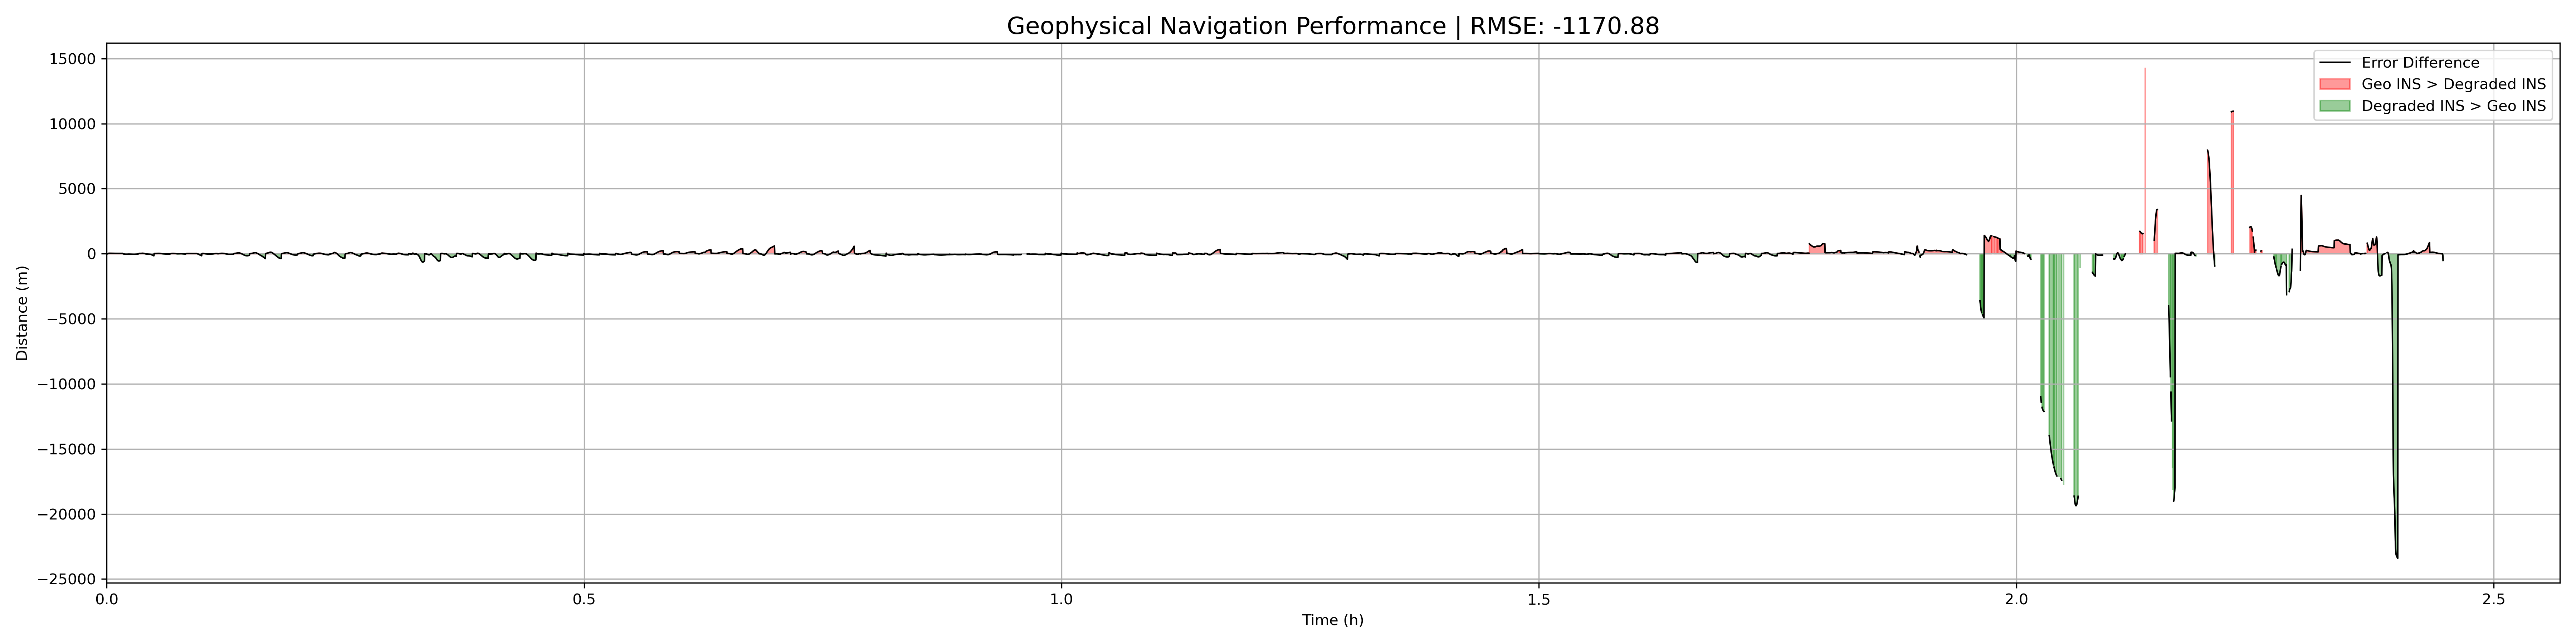
\includegraphics[width=\textwidth]{gravity/2023-08-04_214758_rmse.png}

\vspace{0.3cm}
\textbf{\color{TempleCherry}RMSE Improvement: -1,170 meters}
\end{frame}

% ============================================================
% RESULTS: BEST MAGNETIC PERFORMER
% ============================================================
\begin{frame}{Results: Magnetic Aiding Success}
\centering
\textbf{Trajectory 2025-06-27\_11-54-35}


\includegraphics[width=\textwidth]{magnetic/2025-06-27_11-54-35_rmse.png}

\vspace{0.3cm}
\textbf{\color{TempleCherry}RMSE Improvement: -550 meters}
\end{frame}

% ============================================================
% RESULTS: DUAL-MODAL SUCCESS
% ============================================================
% \begin{frame}{Results: Dual-Modal Performance}
% \centering
% \textbf{Trajectory 2025-07-31\_23-36-03}
% 
% \begin{columns}
% \begin{column}{0.5\textwidth}
% \centering
% 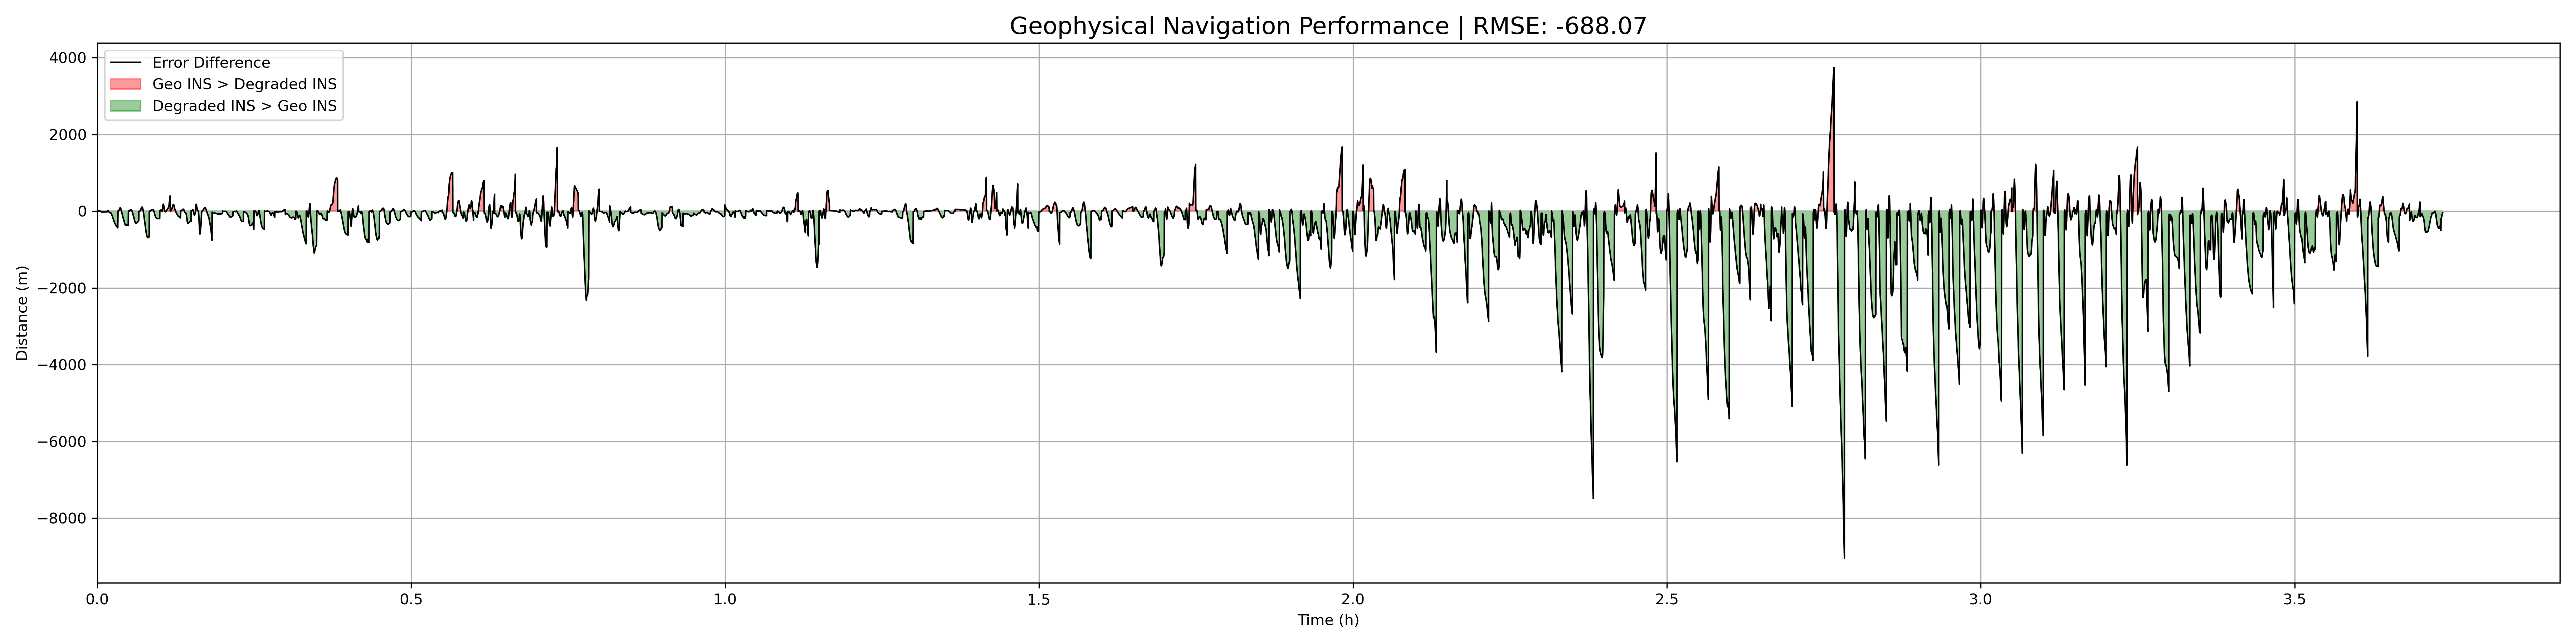
\includegraphics[width=\textwidth]{gravity/2025-07-31_23-36-03_rmse.png}
% \small
% Gravity: -688m RMSE
% \end{column}
% \begin{column}{0.5\textwidth}
% \centering
% 
\includegraphics[width=\textwidth]{magnetic/2025-07-31_23-36-03_rmse.png}
% \small
% Magnetic: -632m RMSE
% \end{column}
% \end{columns}
% 
% \vspace{0.3cm}
% \textbf{\color{TempleCherry}Both modalities provide substantial improvements}
% \end{frame}
% 
% ============================================================
% RESULTS: FAILURE CASE ANALYSIS
% ============================================================
\begin{frame}{Results: Failure Mode Analysis}
\centering
\textbf{Trajectory 2023-08-09\_163741 (Outlier)}

\begin{columns}
\begin{column}{0.5\textwidth}
\centering
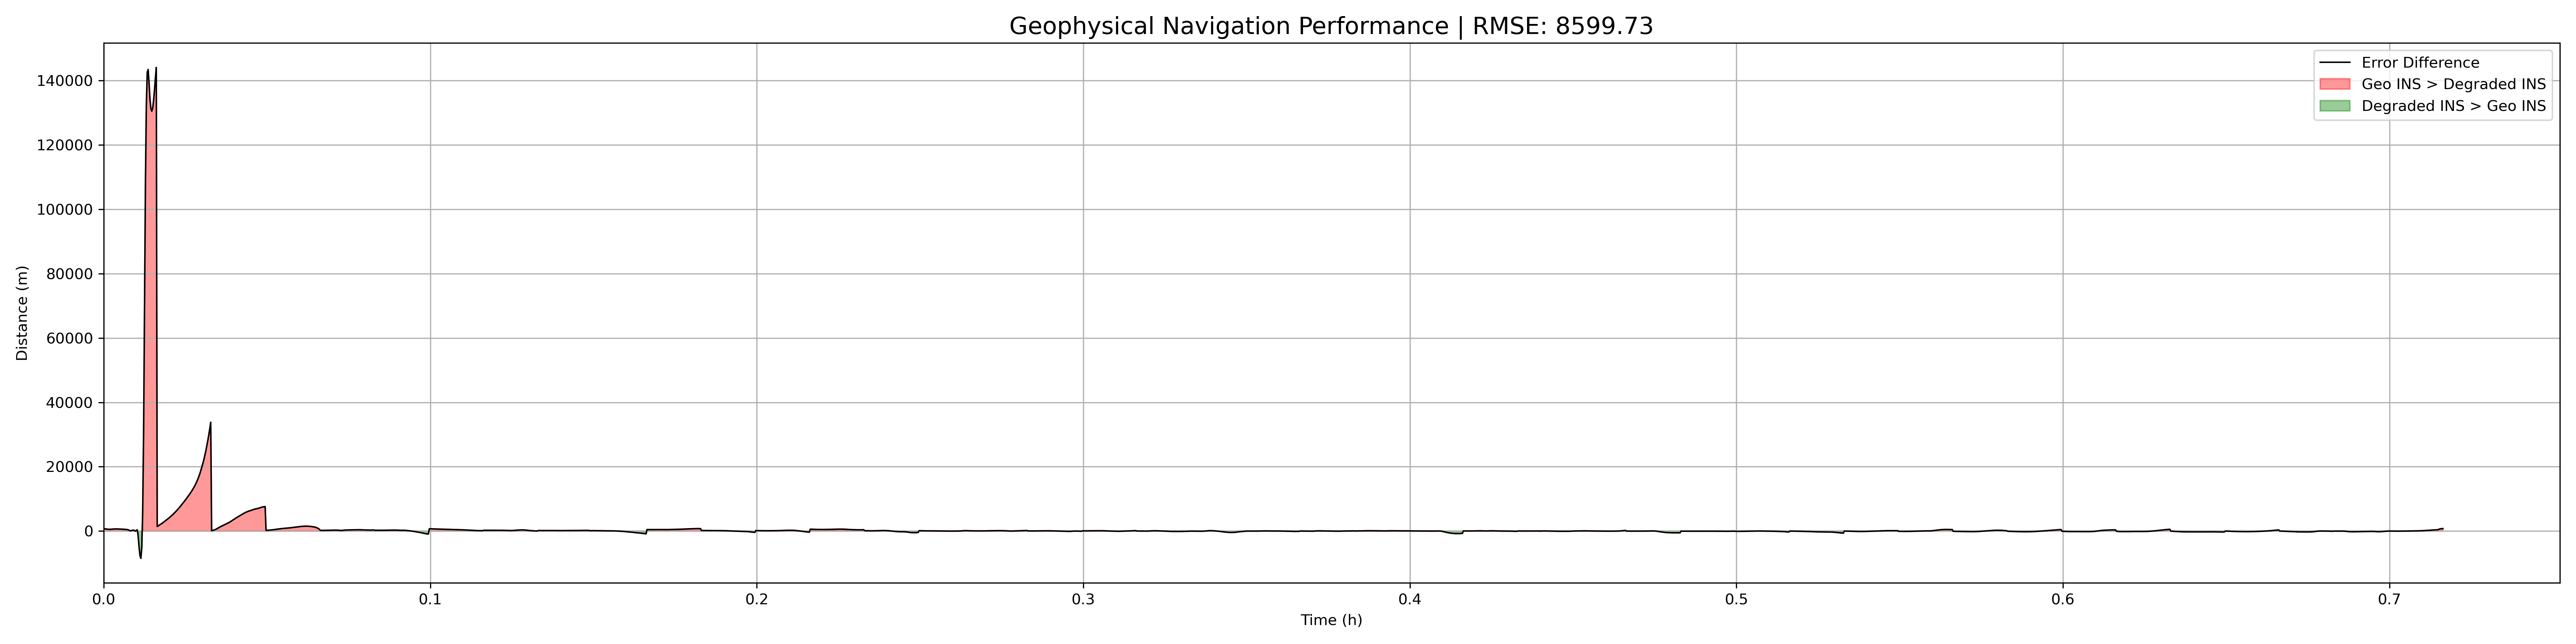
\includegraphics[width=\textwidth]{gravity/2023-08-09_163741_rmse.png}
\small
Gravity: +8,659m error
\end{column}
\begin{column}{0.5\textwidth}
\centering

\includegraphics[width=\textwidth]{magnetic/2023-08-09_163741_rmse.png}
\small
Magnetic: +8,635m error
\end{column}
\end{columns}

\vspace{0.3cm}
\begin{itemize}
    \item Catastrophic initial divergence followed by recovery
    \item Indicates need for integrity monitoring and robust initialization
    \item \textbf{Need:} Improved filter robustness and adaptive measurement weighting
\end{itemize}
\end{frame}

% ============================================================
\section{Discussion}
% ============================================================

% ============================================================
% WHEN DOES IT WORK
% ============================================================
\begin{frame}{When Does Geophysical Aiding Work?}
\begin{columns}[t]
\begin{column}{0.5\textwidth}
\textbf{Success Factors:}
\begin{itemize}
    \item Strong geophysical gradients
    \item Well-mapped regions
    \item Favorable local anomaly characteristics
    \item Complementary modalities (gravity vs magnetic)
\end{itemize}

\vspace{1em}

\textbf{Performance Range:}
\begin{itemize}
    \item Best cases: 100-1,100 m improvement
    \item Typical: 10-100 m improvement
    \item Median errors consistently better
\end{itemize}
\end{column}

\begin{column}{0.5\textwidth}
\textbf{Limitations:}
\begin{itemize}
    \item MEMS sensor noise
    \item Map resolution (1-3 arc-min)
    \item Weak anomaly fields
    \item Filter divergence risk
\end{itemize}

\vspace{1em}

\begin{block}{Key Insight}
Different trajectories benefit from different modalities - multi-modal fusion could improve consistency
\end{block}
\end{column}
\end{columns}
\end{frame}

% ============================================================
% PRACTICAL IMPLICATIONS
% ============================================================
\begin{frame}{Practical Implications}
\textbf{Low-Cost Alt-PNT is Feasible:}
\begin{itemize}
    \item Demonstrated with extremely low-cost MEMS sensors (smartphone-grade)
    \item Using free, publicly available maps
    \item Under severe GNSS degradation
\end{itemize}
\pause
\textbf{Applications:}
\begin{itemize}
    \item Consumer smartphones, electronics, and wearables? \pause \textbf{\textcolor{red}{\texttimes}} \pause
    \item Commercial drones \pause \textbf{\textcolor{green}{\checkmark}} \pause
    \item Small autonomous vehicles \pause \textbf{\textcolor{green}{\checkmark}}
\end{itemize}
\end{frame}

% ============================================================
\section{Conclusion}
% ============================================================

% ============================================================
% KEY TAKEAWAYS
% ============================================================
\begin{frame}{Key Findings}
 %\begin{block}{Primary Achievement}
\textbf{First demonstration of geophysical navigation feasibility using only:}
\begin{itemize}
    \item MEMS-grade sensors
    \item Open-source geophysical maps
    \item Smartphone-class hardware
\end{itemize}
%\end{block}
\pause
\textbf{Performance Highlights}
\begin{itemize}
    \item Error reductions: tens to hundreds of meters on favorable trajectories
    \item Best case: \(\approx\)1,100m RMSE improvement
    \item Median improvements: 3 to 10 meters across all trajectories
    \item Despite MEMS noise and limited map resolution
\end{itemize}
\pause
\textbf{Opens pathway for GNSS-denied geophysical navigation from niche high-end military/aerospace applications to low-SWaP military, aerospace, maritime, and commercial applications.}
\end{frame}

% ============================================================
% FUTURE WORK
% ============================================================
\begin{frame}{Future Directions}
\textbf{Immediate Priorities:}
\begin{enumerate}
    \item \textbf{Multi-Modal Fusion}
    \begin{itemize}
        \item Combine gravity + magnetic measurements
        \item Examine more complex modeling approaches (e.g. Gaussian mixtures, physics informed, etc.)
    \end{itemize}
    \pause
    \item \textbf{Additional Filter Architectures}
    \begin{itemize}
        \item Non-parametric filters (e.g. RBPF, \textit{forthcoming})
        \item EKF vs UKF performance comparison?
    \end{itemize}
    \pause
    \item \textbf{Integrity Monitoring}
    \begin{itemize}
        \item Detect and mitigate failure modes
        \item Adaptive measurement weighting
    \end{itemize}
    \pause
    \item \textbf{Observability Analysis}
    \begin{itemize}
        \item Characterize which regions/trajectories benefit most
        \item Map-matching performance metrics
    \end{itemize}
\end{enumerate}
\end{frame}
% ============================================================
% ACKNOWLEDGMENTS
% ============================================================
\begin{frame}{Acknowledgments}
\textbf{Data Collection Support:}
\begin{itemize}
    \item Beth Brodovsky
    \item Jeremy Brodovsky
    \item Monica Brodovsky
    \item Bill Siegl
    \item Alkesh Kumar Srivastava
\end{itemize}

\vspace{.25cm}

\textbf{Resources:}
\begin{itemize}
    \item MEMS-Nav Dataset: \url{https://doi.org/10.5281/zenodo.17582434}
    \item Strapdown-rs Software: \url{https://github.com/jbrodovsky/strapdown-rs}
    \item IGPP Gravity Anomaly Maps (EGM2008)
    \item World Digital Magnetic Anomaly Map (WDMAM)
    \item Generic Mapping Tools (GMT)
\end{itemize}
\end{frame}

% ============================================================
% Thank you
% ============================================================
\begin{frame}{Thank You!}

\vspace{0.5cm}
\centering
\Large
\textbf{Questions?}

\vspace{0.3cm}
\normalsize
James Brodovsky: jbrodovsky@temple.edu

\vspace{0.5cm}

Brodovsky, J., \& Dames, P. ``Navigation in GNSS-denied environments using MEMS-grade sensors and geophysical anomalies: A UKF approach.'' \textit{ION International Technical Meeting 2026}.
\end{frame}

% ============================================================
% BACKUP SLIDES
% ============================================================
\section{Backup Slides}
\appendix

\begin{frame}[allowframebreaks]{Backup: UKF Algorithm}
\textbf{Unscented Kalman Filter Steps:}

\vspace{0.5em}

\textbf{Sigma Point Generation:}
\begin{equation*}
    \mathcal{X}(\mathbf{x}, \mathbf{P}) =
\begin{cases}
    \mathcal{X}_0 = \mathbf{x} \\
    \mathcal{X}_i = \mathbf{x} + \left( \sqrt{(n + \lambda) \mathbf{P}} \right)_i, & i = 1, \ldots, n \\
    \mathcal{X}_{i+n} = \mathbf{x} - \left( \sqrt{(n + \lambda) \mathbf{P}} \right)_i, & i = 1, \ldots, n
\end{cases}
\end{equation*}

\framebreak

\textbf{Prediction:}
\begin{enumerate}
    \item Generate sigma points: $\mathcal{X}_{t-1}$
    \item Propagate through dynamics: $\bar{\mathcal{X}}_t = g(\mathcal{X}_{t-1}, \mathbf{u}_{t-1})$
    \item Compute predicted mean: $\bar{\mathbf{x}}_t = \sum W^{(m)} \bar{\mathcal{X}}_t$
    \item Compute predicted covariance: $\bar{\mathbf{P}}_t = \sum W^{(c)} (\bar{\mathcal{X}}_t - \bar{\mathbf{x}}_t)(\bar{\mathcal{X}}_t - \bar{\mathbf{x}}_t)^\intercal + \mathbf{Q}$
\end{enumerate}

\textbf{Update:}
\begin{enumerate}
    \item Predict measurements: $\mathcal{Z}_t = h(\mathcal{X}_t)$
    \item Innovation: $\mathbf{y}_t = \mathbf{z}_t - \bar{\mathbf{z}}_t$
    \item Kalman gain: $\mathbf{K}_t = \mathbf{C}_t \mathbf{S}_t^{-1}$
    \item State update: $\mathbf{x}_t = \bar{\mathbf{x}}_t + \mathbf{K}_t \mathbf{y}_t$
\end{enumerate}
\end{frame}

\begin{frame}{Backup: Strapdown Mechanization}
\textbf{Attitude Update:}
\begin{equation*}
\mathbf{C}_{t+1} \approx \mathbf{C}_t \left( I + \boldsymbol{\Omega}_{b} \Delta t \right) - \left( \boldsymbol{\Omega}_{i} + \boldsymbol{\Omega}_{n} \right) \mathbf{C}_t \Delta t
\end{equation*}

\textbf{Velocity Update:}
\begin{equation*}
\mathbf{v}_{t+1} \approx \mathbf{v}_{t} + \left( \hat{\mathbf{f}}_{t} + \mathbf{g}_t - \left( 2\boldsymbol{\Omega}_{i} + \boldsymbol{\Omega}_{n} \right) \mathbf{v}_t \right) \Delta t
\end{equation*}

\textbf{Position Update:}
\begin{align*}
h_{t+1} &= h_{t} + \frac{1}{2} \left( v_{d, t} + v_{d, t+1} \right) \Delta t \\
L_{t+1} &= L_{t} + \frac{1}{2} \left( \frac{v_{n, t}}{R_n + h_t} + \frac{v_{n, t+1}}{R_n + h_{t+1}} \right) \Delta t \\
\lambda_{t+1} &= \lambda_{t} + \frac{1}{2} \left( \frac{v_{e, t}}{(R_e + h_t) \cos L_t} + \frac{v_{e, t+1}}{(R_e + h_{t+1}) \cos L_{t+1}} \right) \Delta t
\end{align*}

\vspace{0.5em}
\small
Reference: Groves, "Principles of GNSS, Inertial, and Multisensor Integrated Navigation Systems," 2nd Ed., Chapter 5
\end{frame}

\end{document}
